\documentclass[11pt]{scrartcl}
\usepackage{fullpage}

\usepackage{cite}
\usepackage{listings} % Coding Syntax coloring
\usepackage{color}
\usepackage{textcomp}
\definecolor{listinggray}{gray}{0.9}
\definecolor{lbcolor}{rgb}{0.9,0.9,0.9}

\usepackage{amsmath}
\usepackage{textcomp}

\usepackage{enumitem}
%\usepackage{hyperref} softeware bug

\lstset{
     backgroundcolor=\color{lbcolor},
     tabsize=4,
     rulecolor=,
     language=matlab,
        basicstyle=\scriptsize,
        upquote=true,
        aboveskip={1.5\baselineskip},
        columns=fixed,
        showstringspaces=false,
        extendedchars=true,
        breaklines=true,
        prebreak = \raisebox{0ex}[0ex][0ex]{\ensuremath{\hookleftarrow}},
        frame=single,
        showtabs=false,
        showspaces=false,
        showstringspaces=false,
        identifierstyle=\ttfamily,
        keywordstyle=\color[rgb]{0,0,1},
        commentstyle=\color[rgb]{0.133,0.545,0.133},
        stringstyle=\color[rgb]{0.627,0.126,0.941},
}
\usepackage{fancyhdr,graphicx,lastpage}% http://ctan.org/pkg/{fancyhdr,graphicx,lastpage}
\fancypagestyle{plain}{
  \fancyhf{}% Clear header/footer
  \fancyhead[R]{
\includegraphics[scale=0.5]{logo.png}}% Right header
  \fancyhead[L]{\textbf{School of Electronic and Electrical Engineering}}
  %\fancyfoot[L]{Name Firstname - v1.0 \\  Date}% Left footer
  \fancyfoot[R]{\thepage\  / \pageref{LastPage}}% Right footer
}
\pagestyle{plain}% Set page style to plain.


\begin{document}
\title{ELEC5563 Individual Project}
\subtitle{ Implementation of Counter, Status Machine, function generator and oscilloscope on the FPGA using Verilog HDL}
\author{Yingjie Luan}
\maketitle

\tableofcontents

\section{Introduction}
\subsection{Objective}
The main objective of this project is to build a digital Oscilloscope based on FPGA using \textit{verilog} language and \textit{Schematic Design}. In general, I am required to read the data from the AD converter and then mapping the data onto monitor via VGA according to a specifically designed timing sequence.
\subsection{Main Aspect}
After one month of works, I have successfully implemented the primary goal, which is to mapping the AD data onto VGA. Not only so, an edge triggering mechanism is implemented for providing a static image, a arbitrary function generator is also implemented as a byproduct of this project. Oscilloscope itself is fully configurable, we can use the switches to control the sample frequency, wave time division, wave center location and wave amplitude. \\

Below is the project result at the functioning result:

\begin{center}
\begin{minipage}[t]{\linewidth}
%\label{fig:main}

{
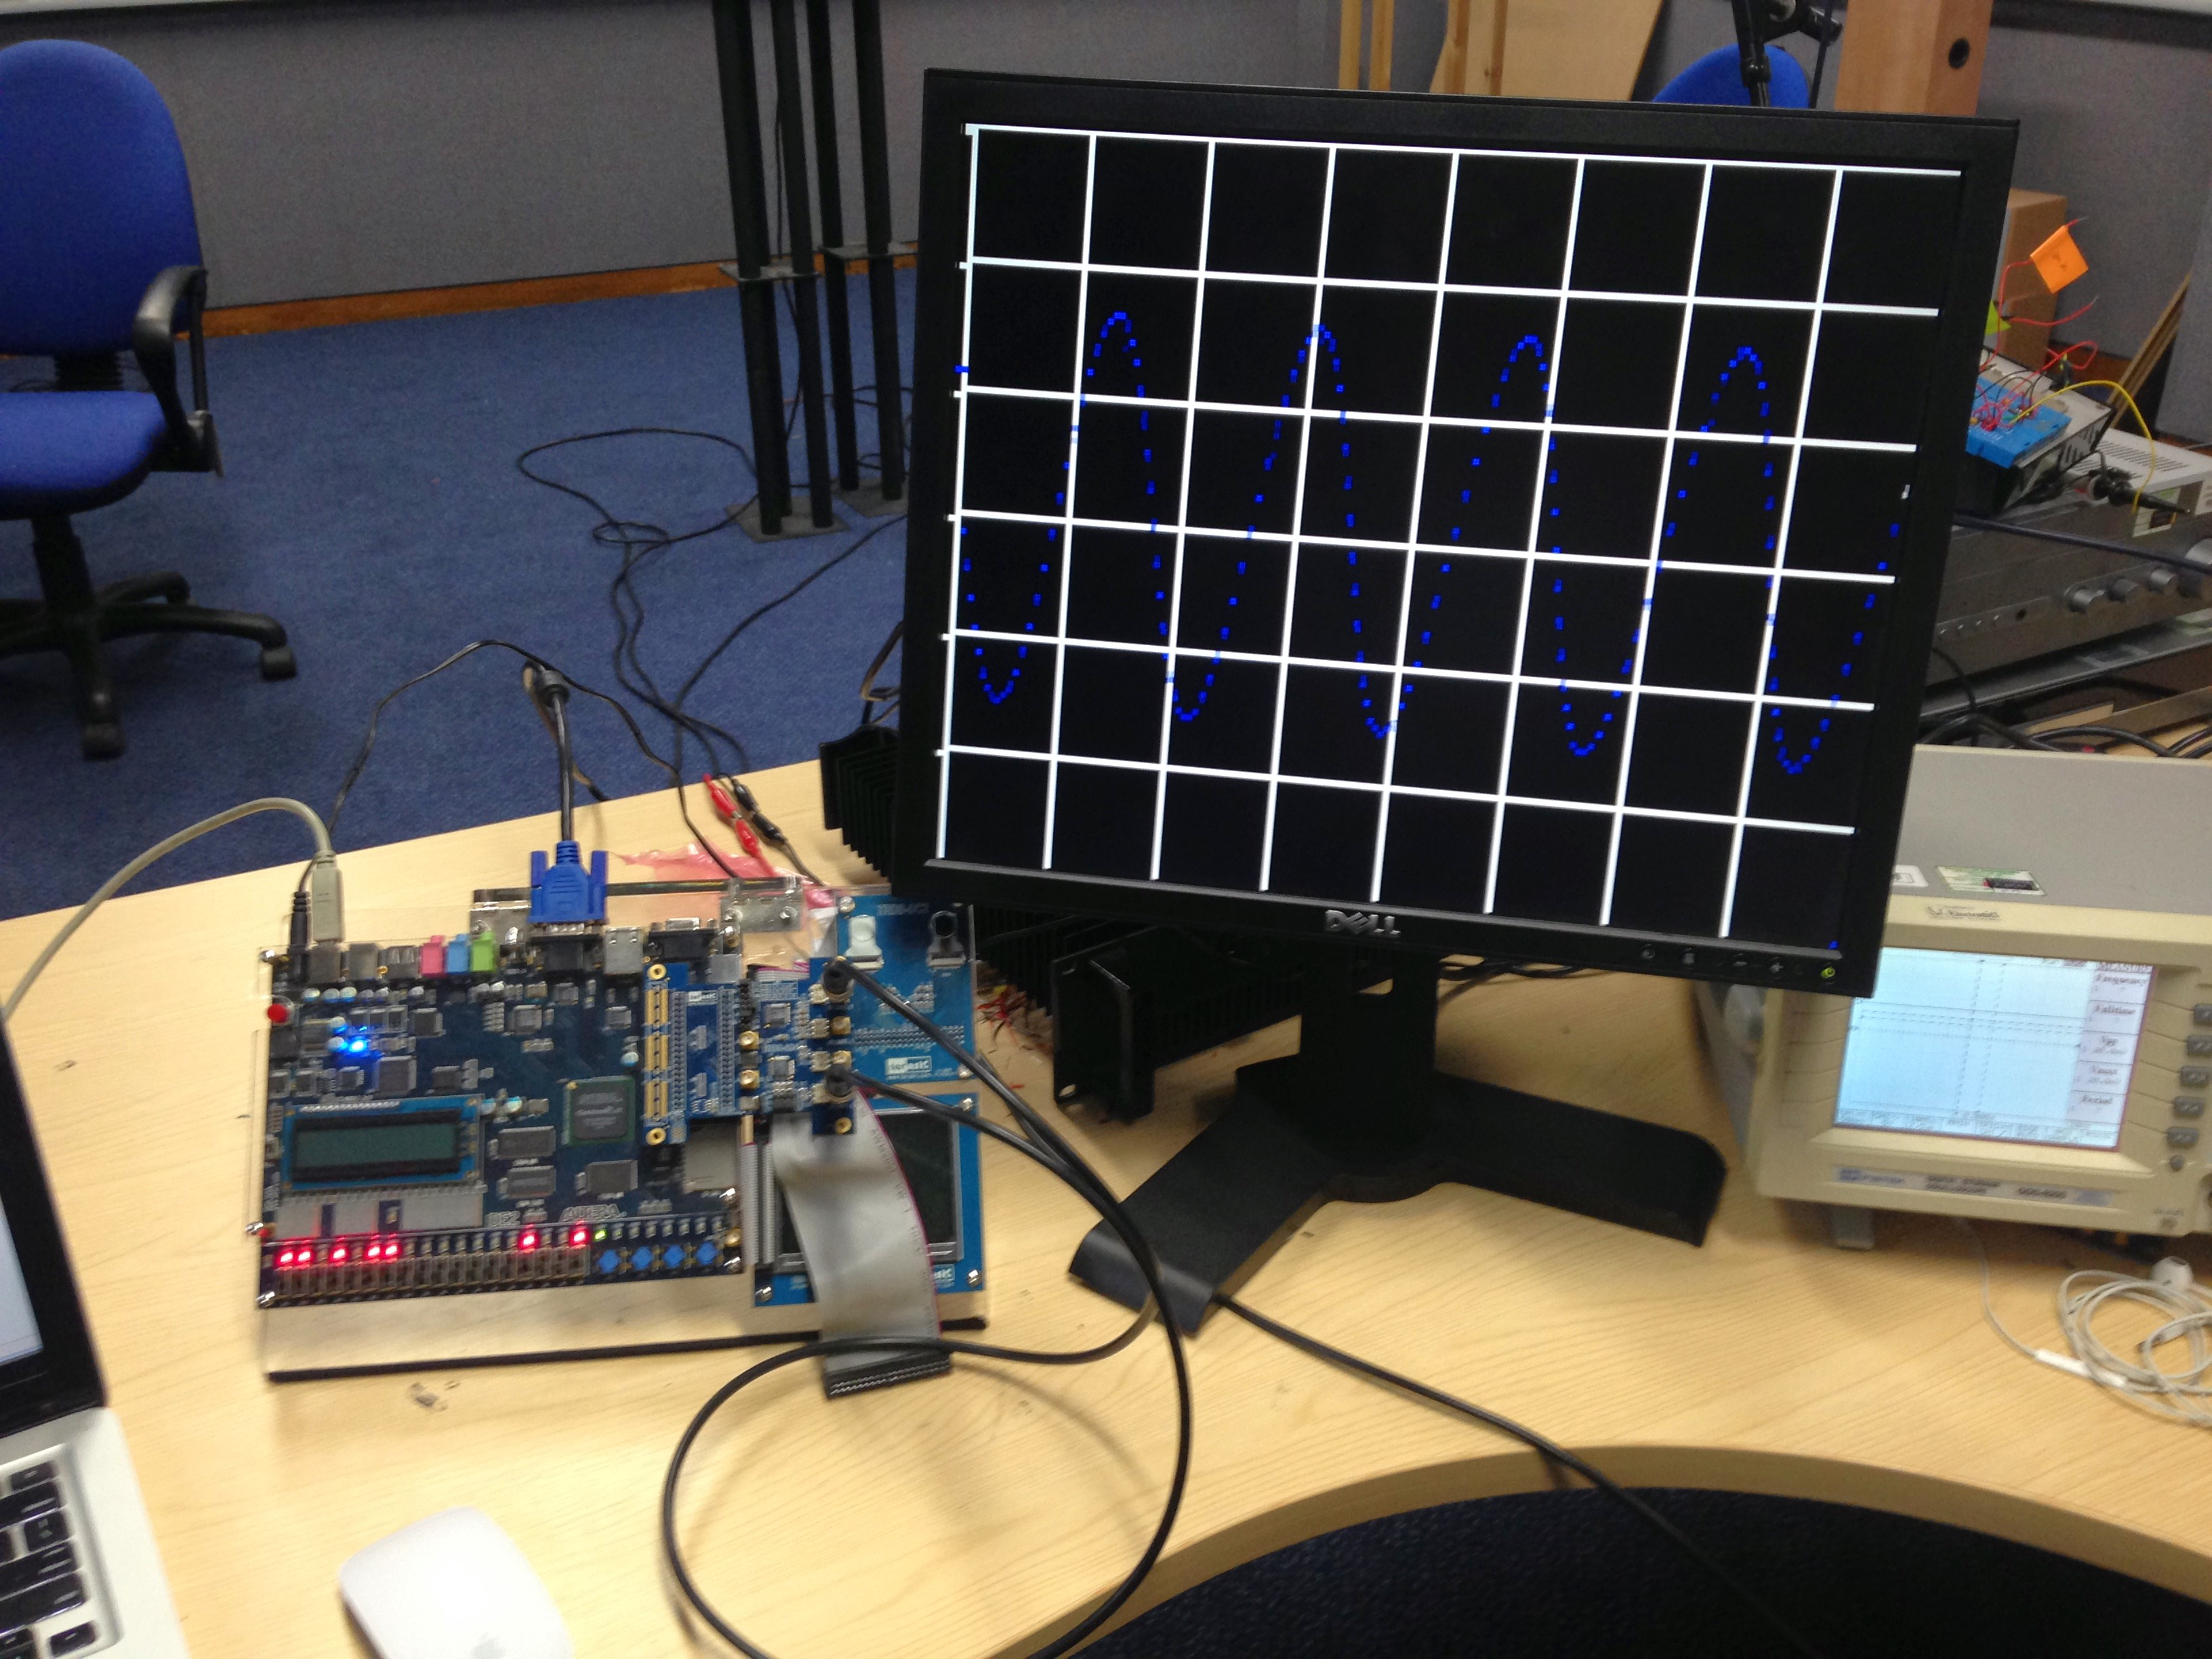
\includegraphics[scale = 0.15]{IMG_1388.JPG}
\captionof{figure}{This is the working result. The oscilloscope is reading the value from the generator}
}
\end{minipage}
\medskip
\end{center}


The board I was working is called \textit{DE2-35}, which is a implementation of the Altera Cyclone\textregistered II FPGA chip 2C35 and the chip code is EP2C35F672C6. The board itself is designed for the purpose of evaluation and education and itself is built in with all sorts of basic components, \textit{i.e.} switches, push button, LCD screen, VGA modulator, GPIO pins etc. Beside from the FPGA board, I also used THDB\_ADA(ADA) daughter board for doing AD and DA conversion. Below is the specification of the chip and the AD-DA daughter board according to \cite{DE2UserManual} and \cite{addaman}.

\paragraph{The technical specification of the AD-DA daughter}

\begin{itemize}
    \item The AD channel is of 14-bit resolution and data rate up to 65 MSPS. Input volage range 2V p-p.
    \item The DA channel is of 14-bit resolution and data rate up to 125 MSPS. Output range 2V p-p.
\end{itemize}

\paragraph{The technical specification of the chip EP2C35F672C6 }
\begin{itemize}
    \item 33,216 LEs
    \item 105 M4K RAM blocks
    \item 483,840 total RAM bits
    \item 35 embedded multipliers
    \item 4PLLs
    \item 475 user I/O pins
    \item FineLine BGA 672-pin package
\end{itemize}

For the software part of the project, a variety of software was used, I used \textit{quartus} for compiling the source code and downloading the program onto the board using JTAG. \textit{Git} for managing the development of the code. \textit{iverilog} for debugging. \textit{Matlab} for doing calculation and generating .mif file. \textit{verilog HDL} is the programming language.\\

The project itself is host at \textit{https://github.com/y1275963/vga\_basics}. With around 24 branches and 80 commits.\\


\section{Board Specification}
\subsection{Board Details}
For the board itself, I implemented a single route oscilloscope at the sampling frequency of 13.5Mhz or 27Mhz or 54Mhz and an arbitary single route capable of generating wave at the base frequency of 97.66Khz and of the data point of 1024 points.%100
\subsection{The controlling method}

Below is the supported control method:

\begin{center}     
\begin{minipage}[t]{\linewidth}
%\label{fig:main}

{
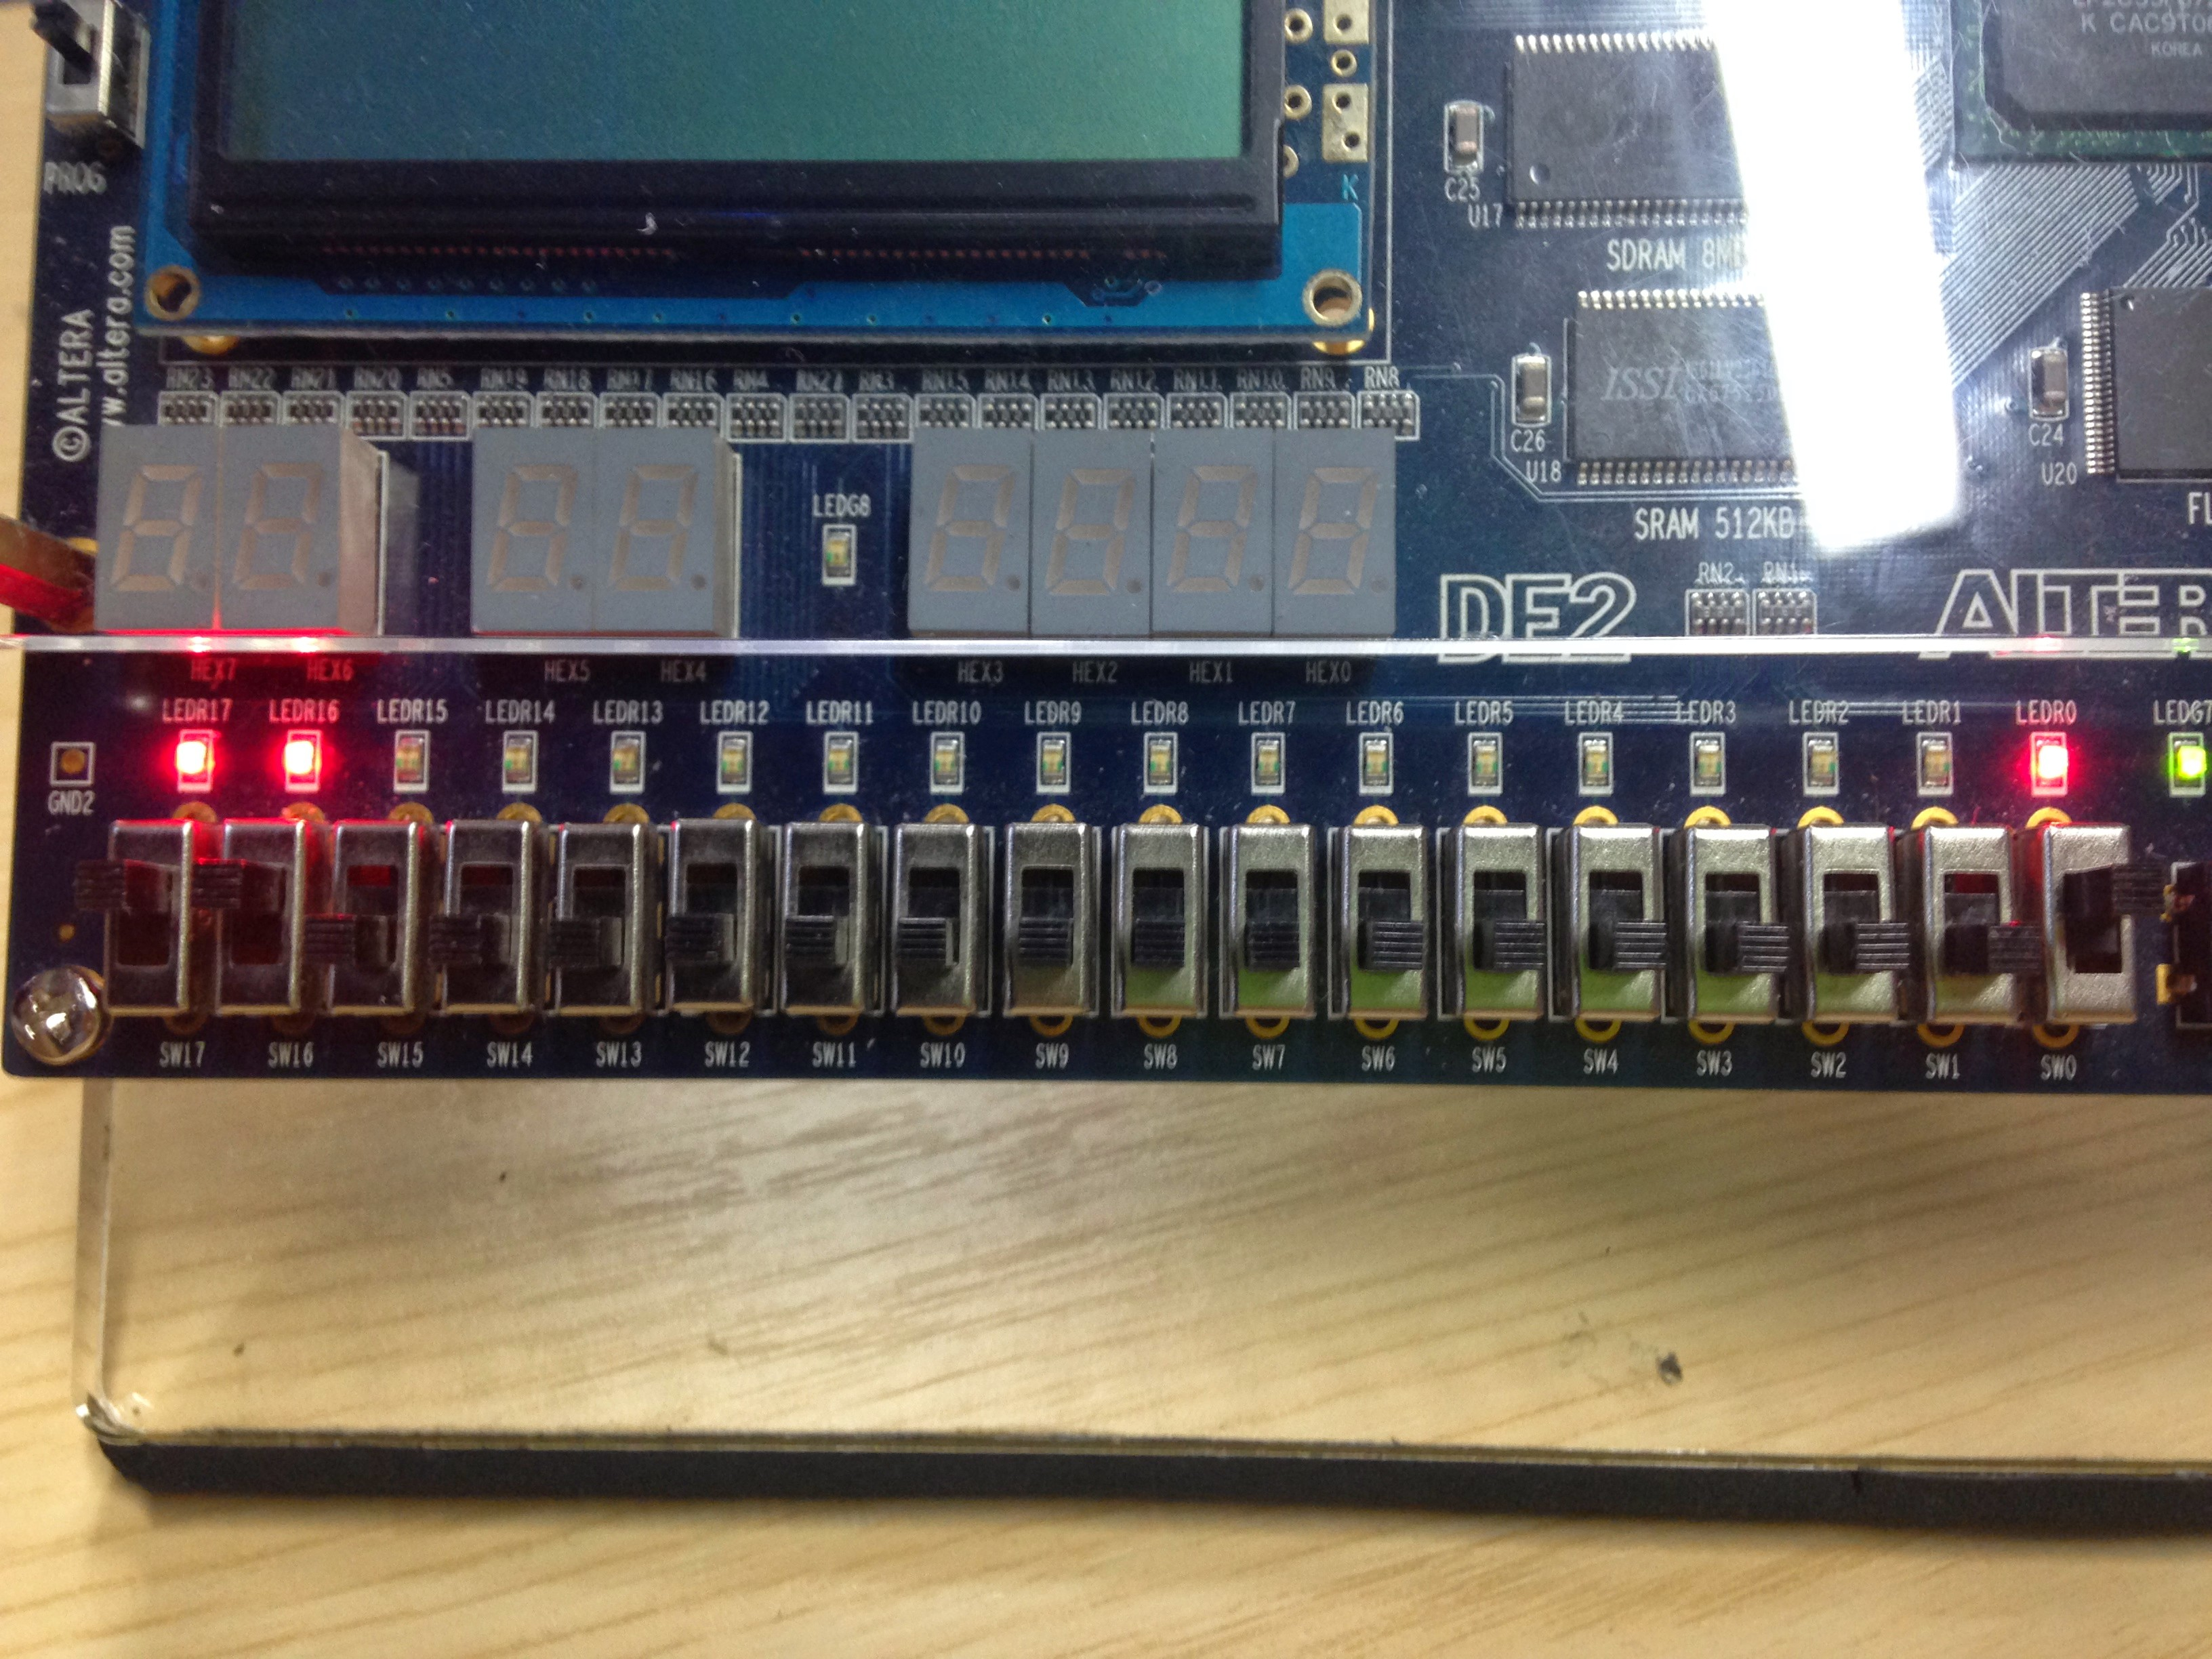
\includegraphics[scale = 0.1]{IMG_1387.JPG}
\captionof{figure}{This is the overall view of the controlling method.}
}
\end{minipage}
\medskip
\end{center}

\begin{itemize}
    \item Switch 17:
    Switch for turning the monitor on or off.
    \item Switch 16:
    Switch for stoping refreshing the screen.
    \item Switch 15:
    Switch for letting the screen only show the background.
    \item Switch 13-14:
    Switch for changing time division by changing sampling frequency.
    
    Specifically:
    \begin{itemize}
        \item Switch 14 on, Switch 13 off:
        Sampling at 13.5Mhz.
        \item Switch 14 off, Switch 13 on:
        Sampling at 54Mhz.
        \item Switch 14 and 13 both on or off:
        Sampling at 27Mhz.        
    \end{itemize}
    \item Switch 11-12:
    Supporting for changing time division by changing sample rate.
    
    Specifically:
    \begin{itemize}
        \item Switch 12 and 11 both off:
        Sample at normal speed.
        \item Switch 12 off and 11 on:
        Sample at 1 time faster normal speed.
        \item Switch 12 on and 11 off:
        Sample at 2 time faster normal speed.
        \item Switch 12 and 11 both on:
        Sample at 3 time faster normal speed.
    \end{itemize}
    \item Switch 8-10:
    Supporting for shift the wave up.
    
    When switch is both off, no shift is made. And by turing it on or off, we can achieve shifting by 1,2,3,4,5,6,7 pixel above the central line.
    \item Switch 5-7:
    Supporting for shift the wave down.
    
    When switch is both off, no shift is made. And by turing it on or off, we can achieve shifting by 1,2,3,4,5,6,7 pixel below the central line.
    \item Switch 1-4:
    Supporting for changing the amplitude of the wave.
    
    The changing of the factor is done by a factor of 2. And switch 4-3 allowing for scale up, switch 2-1 allowing for scale down.
%    Specifically:
%    \begin{itemize}
%        \item Switch 4 and 3 both off:
%        Normal Amplitude.
%        \item Switch 4 off and 3 on:
%        Half of the original amplitude.
%        \item Switch 4 on and 3 off:
%        A quarter of the original amplitude.
%        \item Switch 4 and 3 both on:
%        $\frac{1}{8}$ of the original amplitude.
%    \end{itemize}
    
    \item Switch 0:
    Supporting for turning the function generator on and off.
    
    \item Push button 0:
    Supporting for changing the signal generator generated wave. The design itself allowing the program to record 4 sets of arbitrary waves before compiling the program. (Matlab program is provided for generating such wave) 
\end{itemize}

\subsection{The measuring method}
Below is the supported monitor method to get the data from the board.
\begin{itemize}
    \item The VGA monitor
    
    The monitor is the main source of information. We can use it to see the shape of the wave. Beside from this, because the regular grid is implemented as the background, measurement is made possible. A measurement table is provided for measuring the frequency and the amplitude of the wave. 
    \item The status machine debugger
    \begin{center}     
\begin{minipage}[t]{\linewidth}
%\label{fig:main}

{
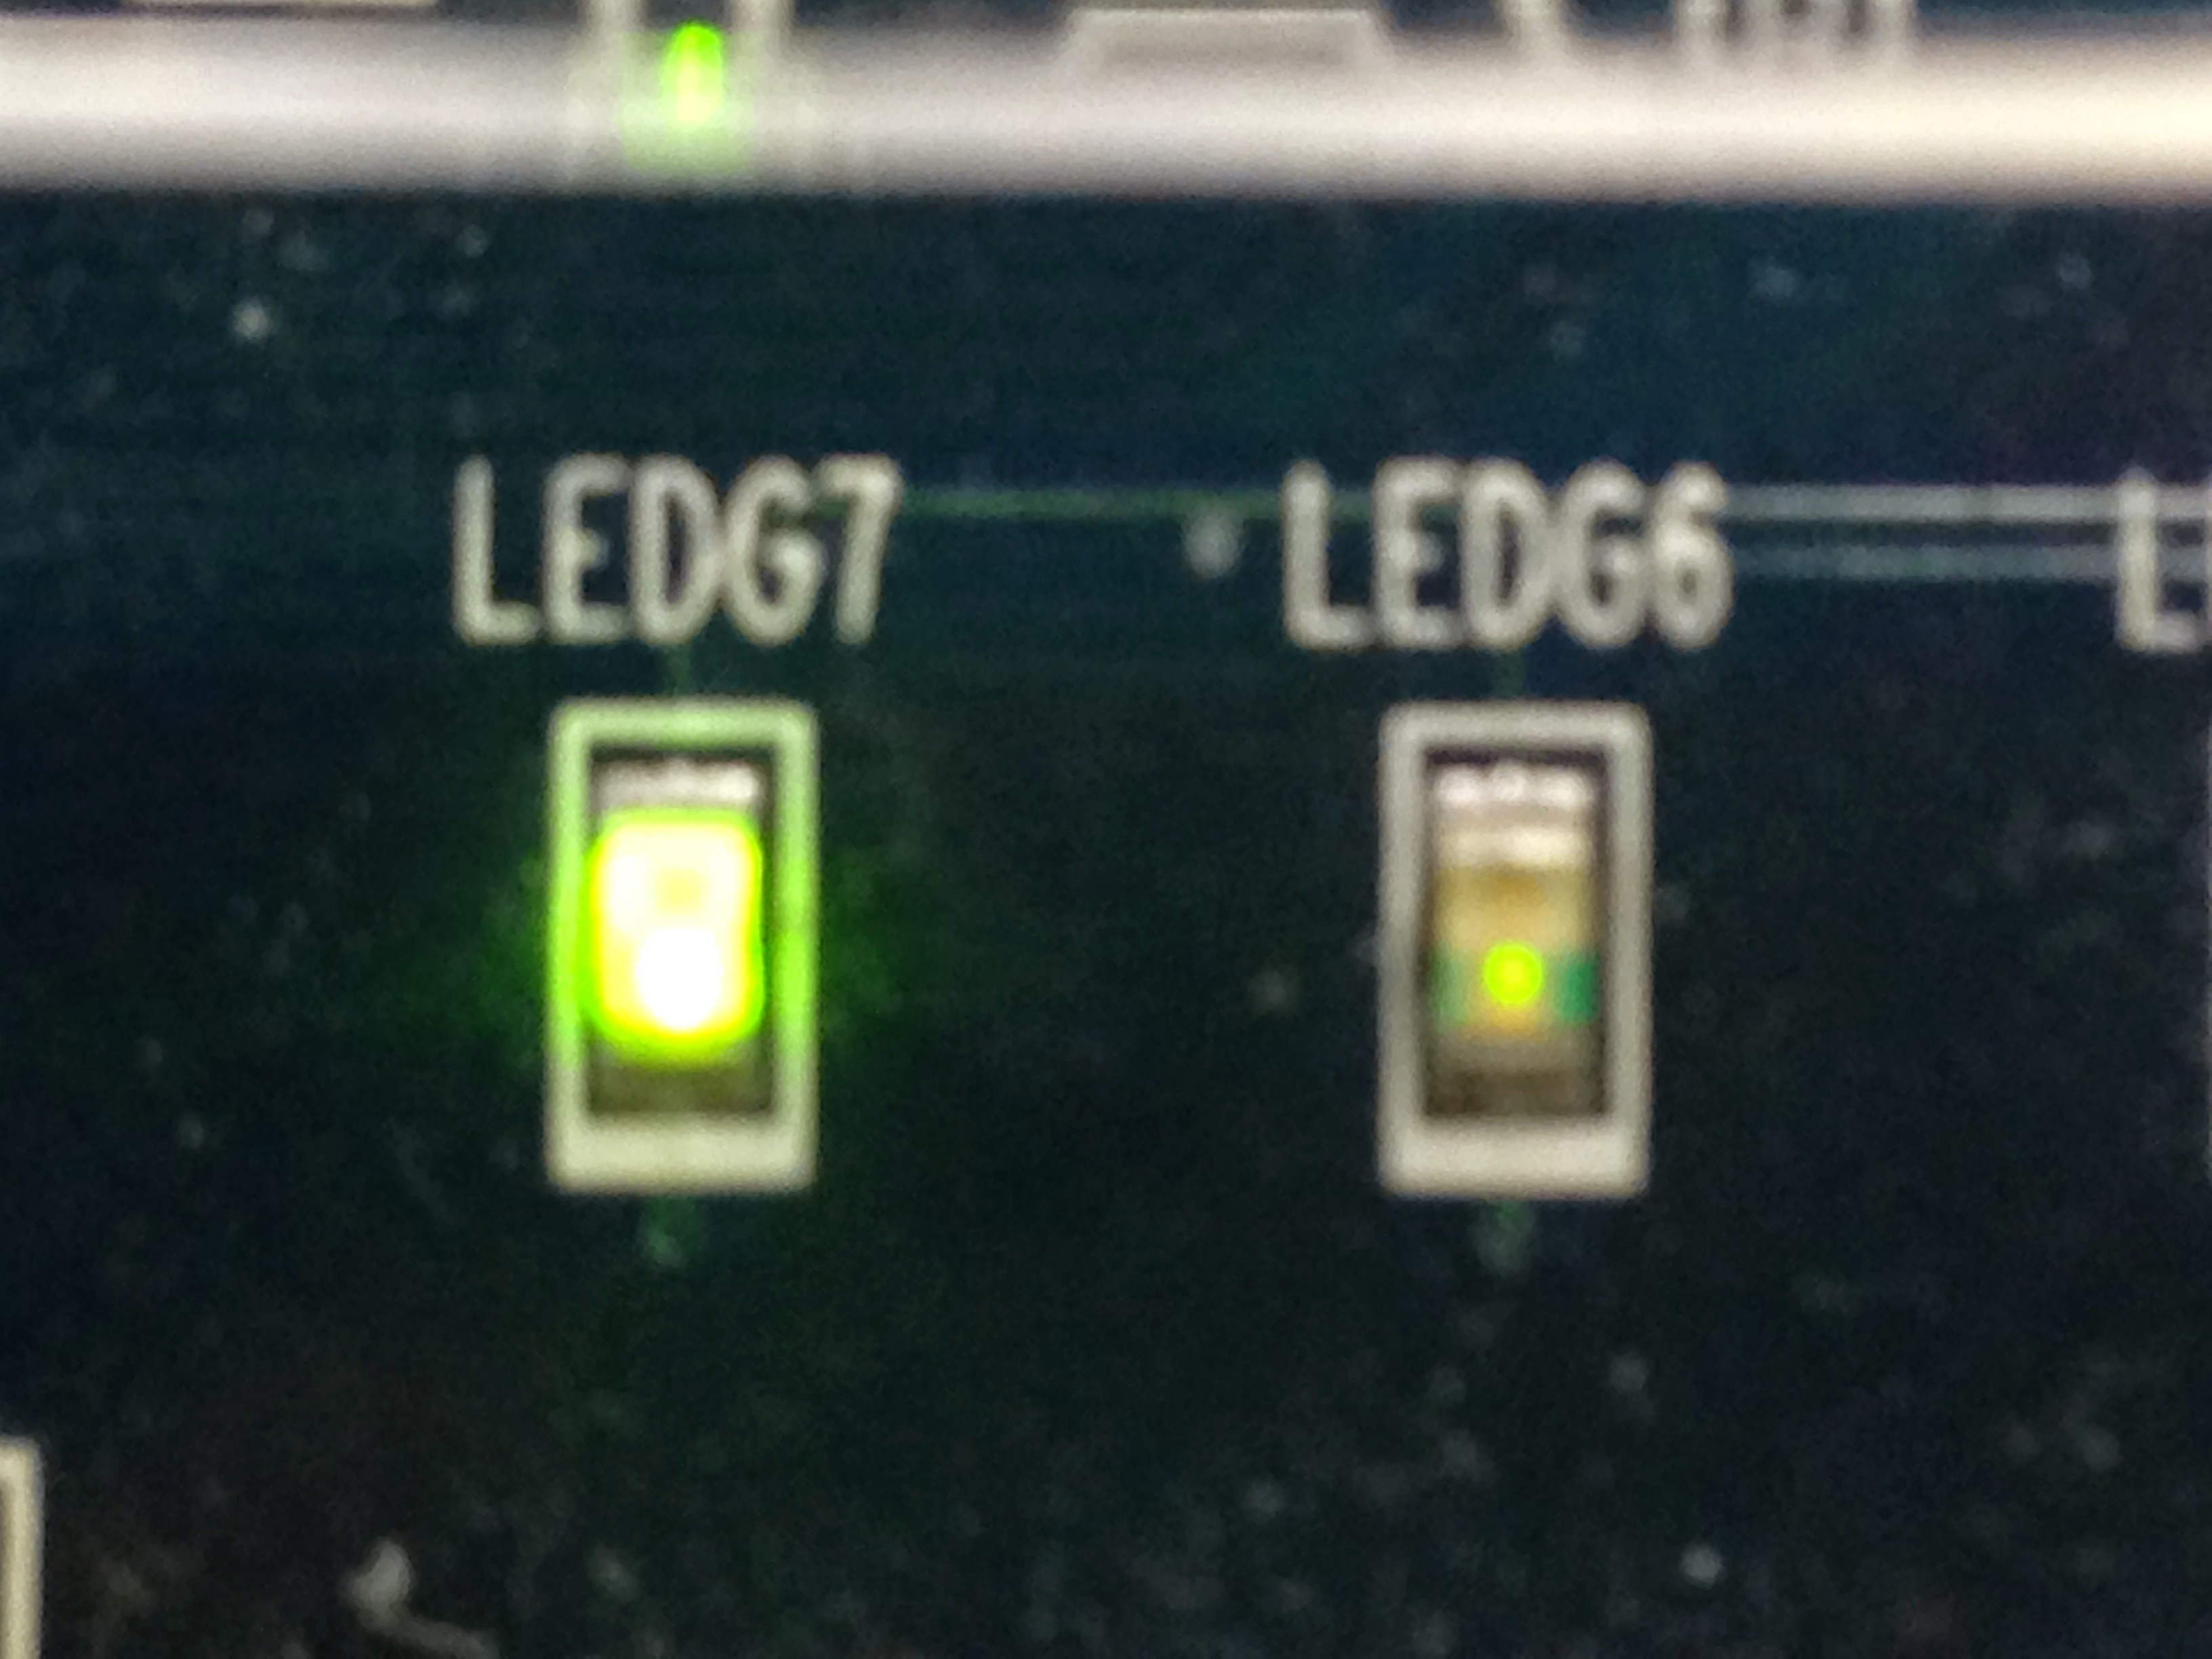
\includegraphics[scale = 0.05]{IMG_1386.JPG}
\captionof{figure}{This is the status indicator.}
}
\end{minipage}
\medskip
\end{center}

     LED Green 7 and 6 are implemented for indicating status machine's current status.( Image blow)

    
    Below is the meaning of the light:
    \begin{itemize}
        \item LED 7 is on, 6 is on, Status 11:
         Meaning that the system is sampling from the AD convert.
         \item LDE 7 is on, 6 is off, Status 10:
         Meaning that the system is delayed, to moderate the refresh rate down to around 50hz.
         \item LED 7 is off, 6 is on, Status 01:
         Meaning that the system is drawing the wave from the Ram according to the sampled signal.
         \item LED 7 is off, 6 is off, Status 00:
         Meaning that the system is clean the screen by redrawing a regular grid background.
    \end{itemize}  
    
    In reality, as we can see from the image above, because the system is delayed for most of its functioning time, we can see LED 7 is always on, and LED 6 is glimmering. Which means the system spent most of its time in delaying(Status 10).
    
      
\end{itemize}

\subsection{The workflow}

This is the overall schematic chart:
\begin{center}
\begin{minipage}[t]{\linewidth}
%\label{fig:main}

{
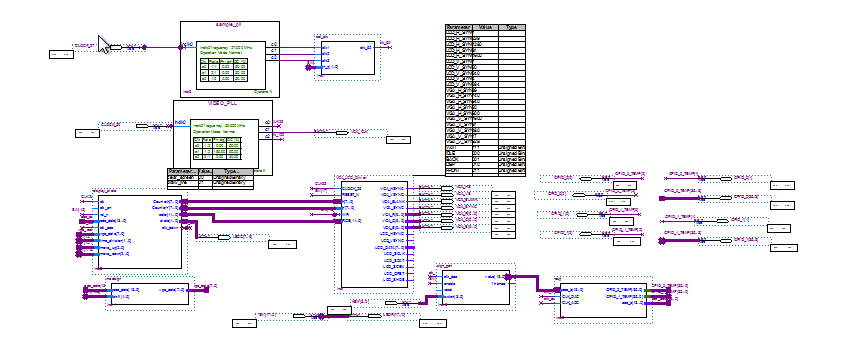
\includegraphics[scale = 0.5]{schematic.png}
\captionof{figure}{This is the workflow of the oscilloscope.}
}
\end{minipage}
\medskip
\end{center}

The board will execute two job simultaneously, below is the flowchart of the Oscilloscope:

\begin{center}
\begin{minipage}[t]{\linewidth}
%\label{fig:main}

{
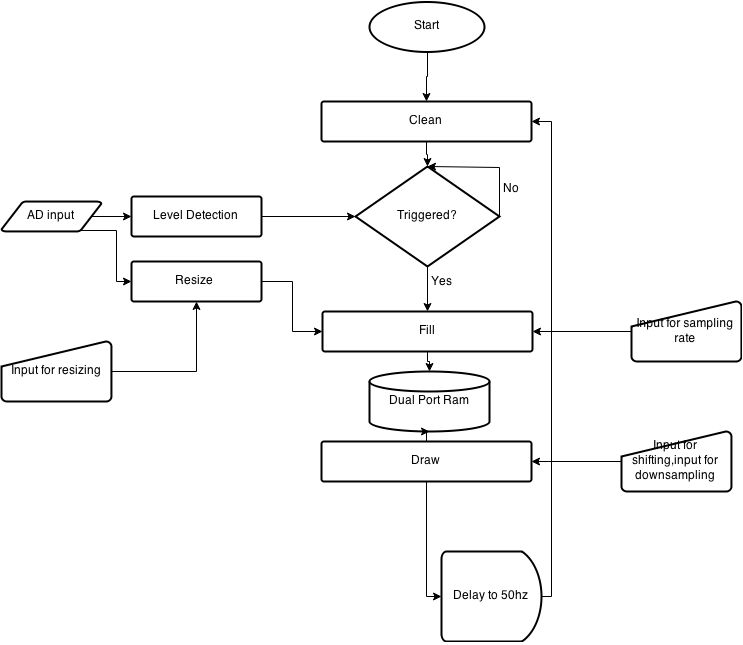
\includegraphics[scale = 0.5]{adchar.png}
\captionof{figure}{This is the workflow of the oscilloscope.}
}
\end{minipage}
\medskip
\end{center}
Below is the flowchart of the arbitrary function generator:
\begin{center}
\begin{minipage}[t]{\linewidth}
%\label{fig:main}

{
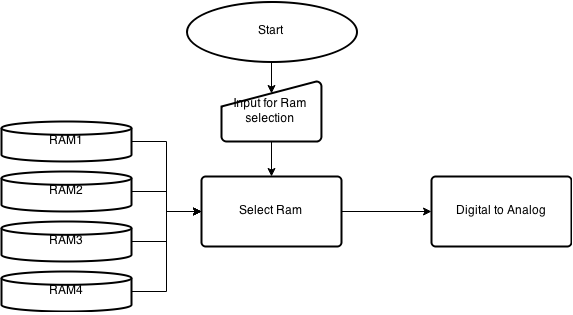
\includegraphics[scale = 0.6]{dachart.png}
\captionof{figure}{This is workflow of the function generator.}
}
\end{minipage}
\medskip
\end{center}


\section{Implementation Details}
\subsection{The Counter}
The counter is the building block of the entire project and it is used throughout the entire project. Below is the detailed list of the usage of the counter:
\begin{itemize}
    \item In Drawing process:
     Counters are used to provide VGA the pixel coordinates.
     \item In delay process:
     Counter is used to crate a delay to lower down the refresh rate.
     \item In Sampling process and AD process:
    Counter is used to provide the Ram with memory index. A counter in sampling process also support downsampling the Ram.
\end{itemize}

To connect counters with status machine, all the counter is implemented 2 input signals and 1 output signal:
\begin{itemize}
    \item enable: To start the counter
    \item reset: To reset the counter
    \item finished: indicate if the counter has finished one round or not.
\end{itemize}
\subsubsection{The basic Counter}
All the counters are built on top the basic structure from the one blow:

\begin{lstlisting}[language=Verilog]
input clk;
input enable,reset;

output finished;
output reg [7:0] CounterX;
wire CounterXmaxed = (CounterX==8'd159); 
assign finished = (CounterXmaxed==1);

always @(posedge clk)
begin
	if(reset == 1)
		CounterX <= 0;
	else
	begin
	if(CounterXmaxed)
	  	CounterX <= 0;
	else if(enable == 1)
	  	CounterX <= CounterX + 1;
	 end
end
\end{lstlisting}

By setting the value of the maximum value of the counter, we can manage to let the counter counts from 0 to its max value according to the clock. And the finished signal is emitted right at the moment the counter reach its maximum value.

\subsubsection{Jumping Counter}
The downsampling is implemented by downsampling the output of the Ram instead of downsampling the output from the AD convert from the simple fact the the system can endure a little bit more delay.(Moreover, an explicit delay is implemented).

To support the downsampling, we simply change the increment factor of the counter and hence we change the Ram address we are going to access, below is an example of the jumping counter:
 
\begin{lstlisting}[language=Verilog]
input [1:0] time_division;
wire [2:0] read_time_division = time_division + 1; // to avoid 0, start from 1

output reg [7:0] read_CounterX;

wire read_CounterX_Maxed = (read_CounterX >= 8'd1023);

always @(posedge clk)
begin
	if(reset == 1)
		read_CounterX <= 0;
	else
	begin
	if(read_CounterX_Maxed)
	  	read_CounterX <= 0;
	else if(enable == 1)
	  	read_CounterX <= read_CounterX + read_time_division + 1;
	 end
end
\end{lstlisting}
\subsubsection{Counter on top of the Counter}
To support providing $(x,y)$ coordinators for the VGA module while cleaning the whole screen, a Y counter is built on top of a X counter, blow is the example:
\begin{lstlisting}[language=Verilog]

input clk;
input reset,enable;

output reg [7:0] CounterX,CounterY;
output finished;

wire [14:0] address;

wire CounterXmaxed = (CounterX==8'd159); // 159
wire CounterYmaxed = (CounterY==8'd119); // 119
assign finished = ((CounterXmaxed == 1) && (CounterYmaxed == 1));

assign address = CounterX + CounterY * 160;

always @(posedge clk)
begin
	if(reset == 1)
		CounterX <= 0;
	else
	begin
	if(CounterXmaxed)
	  CounterX <= 0;
	else if(enable == 1)
	  CounterX <= CounterX + 1;
	end
end

always @ (posedge clk)
begin
	if(reset == 1)
		CounterY <= 0;
	else
	begin
		if(CounterXmaxed == 1)
\end{lstlisting}
\subsubsection{iverilog output for testing}
Because we need a reliable counter to make sure it goes exactly as we wish, \textit{iverilog} is used for testing, below is its output:

This is snapshot of the testing from the basic counter:
\begin{verbatim}
ticket:23370    ,enable:1       ,reset:0        ,x:155  ,finished :0
ticket:23380    ,enable:1       ,reset:0        ,x:156  ,finished :0
ticket:23390    ,enable:1       ,reset:0        ,x:157  ,finished :0
ticket:23400    ,enable:1       ,reset:0        ,x:158  ,finished :0
ticket:23410    ,enable:1       ,reset:0        ,x:159  ,finished :1
ticket:23420    ,enable:1       ,reset:0        ,x:  0  ,finished :0
\end{verbatim}
Below is the snapshot of the testing from the jumping counter:
\begin{verbatim}
ticket:23950    ,enable:1       ,reset:0        ,x:147  ,finished :0
ticket:23960    ,enable:1       ,reset:0        ,x:150  ,finished :0
ticket:23970    ,enable:1       ,reset:0        ,x:153  ,finished :0
ticket:23980    ,enable:1       ,reset:0        ,x:156  ,finished :0
ticket:23990    ,enable:1       ,reset:0        ,x:159  ,finished :1
ticket:24000    ,enable:1       ,reset:0        ,x:  0  ,finished :0
ticket:24010    ,enable:1       ,reset:0        ,x:  3  ,finished :0
ticket:24020    ,enable:1       ,reset:0        ,x:  6  ,finished :0
\end{verbatim}


Below is the snapshot of the testing from the xy counter:
\begin{verbatim}
ticket:575970   ,enable:1       ,reset:0        ,x:155  ,y:119  ,finished :0
ticket:575980   ,enable:1       ,reset:0        ,x:156  ,y:119  ,finished :0
ticket:575990   ,enable:1       ,reset:0        ,x:157  ,y:119  ,finished :0
ticket:576000   ,enable:1       ,reset:0        ,x:158  ,y:119  ,finished :0
ticket:576010   ,enable:1       ,reset:0        ,x:159  ,y:119  ,finished :1
ticket:576020   ,enable:1       ,reset:0        ,x:  0  ,y:  0  ,finished :0
ticket:576030   ,enable:1       ,reset:0        ,x:  1  ,y:  0  ,finished :0
ticket:576040   ,enable:1       ,reset:0        ,x:  2  ,y:  0  ,finished :0
ticket:576050   ,enable:1       ,reset:0        ,x:  3  ,y:  0  ,finished :0
\end{verbatim}

Below is the example of the test bench:
\begin{lstlisting}[language=Verilog]
module ramfill_tb;

// module ramfill(clk_adc,enable,reset,finfished,adc_data,vga_data,CounterX);
reg clk;
wire [7:0] CounterX;
reg enable,reset;
wire finished;

vga_sin u0(
	.clk(clk), 
	.reset	(reset),
	.enable (enable),
	.finished (finished), 
	.CounterX	(CounterX));

always  
   #5 clk = ~clk; 
    
initial begin
	reset = 0;
	enable = 0;
	clk = 1;

	#10 reset = 1;//after 10 tickets
	#10 reset = 0;//then after 10 tickets,reset is set 1 after reset == 1 is kept for 10 tickets
	#10 enable = 1;
	#20000 reset = 1;//try again
	#200 reset = 0;
	#2000 enable = 1;
	#2000 enable = 0;
	#200 reset = 0;
	#25 $finish; 
end


initial  begin
    $monitor("ticket:%g\t,enable:%b\t,reset:%b\t,x:%d\t,finished :%b",$time,enable,reset,CounterX,finished); 
end 

endmodule
\end{lstlisting}

\subsection{The RAM}
It would be good if we can write some test bench with Ram, but because it is a Mega function and I cannot find a way to compile it.


The Ram is used throughout the project as well, below is a list of its usage:
\begin{itemize}
    \item In clean process: A Ram is used to provide the image of the grid which is going to be drawn.
    \item In sampling process: A Ram is used to store the sampling information
    \item In drawing process: The same Ram is used to retrieve information from the Ram.
    \item In DA process: 4 Rams are used to store the pro recored wave information. 
    \end{itemize}
\subsubsection{One Port reading only RAM}
This is the basic usage of the Ram, and the purpose of this is simply to get the initialing memory information from the Ram, below is an example:
\begin{lstlisting}[language=Verilog]
wire rambuffer;
ram_background ram_entity(
 	.address(address),
 	.clock(clk),
 	.wren(1'b0),
 	.q(rambuffer));
endmodule
\end{lstlisting}
And we just get the information from the address which is defined by our counter.

\subsubsection{Dual Port RAM}

That is hardest part of the entire project, and the natural way of doing so is by using a FIFO mega function \cite{fifo}. But because \textit{quartus} only provide fixed length FIFO and due to various other reasons, I cannot figure out a right way of stopping the FIFO from overflow, an image is provided to demonstrate the problem:


\begin{minipage}[t]{\linewidth}
%\label{fig:main}

{

\includegraphics[scale = 0.3]{apr.jpg}
\captionof{figure}{There is a periodic unsolvable overflow problem at each image.}
}
\end{minipage}
\medskip

And a dual port asynchronous memory is a core component of the entire design, it is used to link the AD sampled data to the image on the screen. Its difficulties are listed as follows:
\begin{itemize}
    \item It must support one reading port and one writing port running at different speed.
    \item It is written at writing speed, but at the reading cycle the finishing of the writing must be able to be detected. And the clock shift is unknown. 
    \item There is a trigging mechanism in between, so the port is not being written periodically.
\end{itemize}

And the solution is the example below:
\begin{lstlisting}[language=Verilog]
// sync clocks
reg prolong_finished = 0;
always @(posedge w_finished) // flip flop
begin
	prolong_finished = prolong_finished + 1;
end

reg previous_signal;
reg r_finished;
always @(posedge clk) 
begin
	previous_signal <= prolong_finished; 
	r_finished <= previous_signal ^ prolong_finished;
	// or with its previous value.
end
\end{lstlisting}

The writing finished signal will change the status of a flip-flop register, and the reading clock will be constantly detecting the level of the register and when  it detects the difference it will output a reading finished signal.

By doing so, I successfully made the writing finished clock readable from the reading cycle. Therefor, at the status machine it will be able to detect if the sampling is finished at a different clock.\\


Below is a simulation result:

\begin{minipage}[t]{\linewidth}
%\label{fig:main}

{
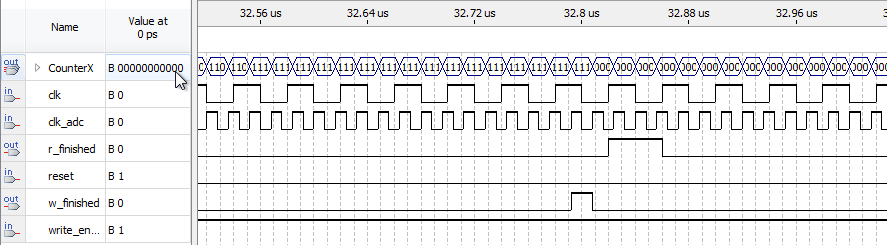
\includegraphics[scale = 0.5]{dualram.png}
\captionof{figure}{This is simulation of the synchronization of the finished clock.}
}
\end{minipage}
\medskip

\subsection{The Status Machine}
The status machine runs at the pixel refresh rate, which is 25Mhz, and it is the main block of the whole project. \\


The implementation of status machine goes as the following, Whenever a status's mission is finished it will define a next state. And there is a cycle to change the status according. 

For all the status, it always goes from enabling its module and reseting all the rest modules. \\


It is separated in 4 stages:
\begin{itemize}
    \item clean:
    Call the clean module to clean the screen, and wait until it is finished.
    \item fill:
    Call the Sampling module to write memory to the Ram, and wait until it is finished. Notice that the status machine detects the status of the filling module at 25Mhz but the filling module itself runs at sampling frequency.
    \item draw:
    Call the drawing module to draw the memory from the Ram, and wait until it is finished.
    \item delay:
    Call the delay module to delay the whole process, and wait until it is finished.
\end{itemize}




Below is the snapshot code of the status machine:
\begin{lstlisting}[language=Verilog]

always @ (posedge clk)
begin
	if(rst_n == 1)
		state <= clear_screen;
	else
		state <= next_state;
end

always @ * // combinational circuit
	case(state)
		clear_screen:
		begin
			enable_clear = 1;
			reset_clear = 0;

			enable_sin = 0;
			reset_sin = 1;

			enable_delay = 0;
			reset_delay = 1;

			enable_fill = 0;
			reset_fill = 1;

			CounterX = CounterX_clear;
			CounterY = CounterY_clear;
			color = color_clear;
			if(finished_clear == 0)
				next_state = clear_screen;
			else
				next_state = fill;
		end
		fill:
		begin
			enable_fill = 1;
			reset_fill = 0;		

			enable_clear = 0;
			reset_clear = 1;

			enable_sin = 0;
			reset_sin = 1;

			enable_delay = 0;
			reset_delay = 1;

			CounterX = 8'bzzzz_zzz;
			CounterY = 8'bzzzz_zzz;
			color = 12'bzzz_zzz_zzz_zzz;

			if(finished_fill == 0)
				next_state = fill;
			else
				next_state = draw_line;			

		end
		draw_line:
		begin
			enable_sin = 1;
			reset_sin = 0;

			enable_delay = 0;
			reset_delay = 1;

			enable_clear = 0;
			reset_clear = 1;

			enable_fill = 0;
			reset_fill = 1;			

			CounterX = CounterX_sin;
			CounterY = ram_output + move_down - move_up;
			color = color_sin;
			if(finished_sin == 0)
				next_state = draw_line;
			else
				next_state = do_nothing;
		end
		do_nothing:
		begin
			enable_delay = 1;
			reset_delay = 0;

			enable_clear = 0;
			reset_clear = 1;

			enable_sin = 0;
			reset_sin = 1;

			enable_fill = 0;
			reset_fill = 1;			

			CounterX = 8'bzzzz_zzz;
			CounterY = 8'bzzzz_zzz;
			color = 12'bzzz_zzz_zzz_zzz;
			if(finished_delay == 0)
				next_state = do_nothing;
			else	
				next_state = clear_screen;
		end 
	endcase
\end{lstlisting}
 
\subsection{The Trigger}

The trigger detects the input signal and emit an enabling signal to start the sampling, two mechanism is implemented and tested.


The first one is simply to use the most significant bit of the input signal:

\begin{lstlisting}[language=Verilog]
wire last_bit_data = adc_data[13];
reg previous_adc_data;
// wait until trigger happen
always @ (posedge clk_adc)
begin
	previous_adc_data <= last_bit_data;
	if(enable == 1)
	begin
		if((last_bit_data ^ previous_adc_data) == 1) // unchanged until enable returns to 0.
			write_enable <= 1;
	end
	else
		write_enable <= 0;
end
\end{lstlisting}

and according to \cite{trigger}, I implemented a different design:

\begin{lstlisting}[language=Verilog]

always @ (posedge clk_adc)
begin
	if(enable == 1)
	begin
		if(Trigger == 1) // unchanged until enable returns to 0.
			write_enable <= 1;
	end
	else
		write_enable <= 0;
end

reg Threshold1, Threshold2;
always @(posedge clk_adc) Threshold1 <= (adc_data>=14'b10_000_000_000_000);
always @(posedge clk_adc) Threshold2 <= Threshold1;

wire Trigger = Threshold1 & ~Threshold2;  // if positive edge, trigger! 
\end{lstlisting}

Both of the design work, but according to the performance, the last one works better than the former.\\

Clearly, we can pin out the \textit{trigger} signal and therefor enable the external trigger signal.
\subsection{PLL}

PLL is used to change the clock, two PLLs are implemented,

The first one receive signal from 50Mhz and generate 3 signals. Two for VGA module, which are 25Mhz and 25Mhz with 180 degree shift. One for DA module which is 100Mhz.

\begin{minipage}[t]{\linewidth}
%\label{fig:main}

{
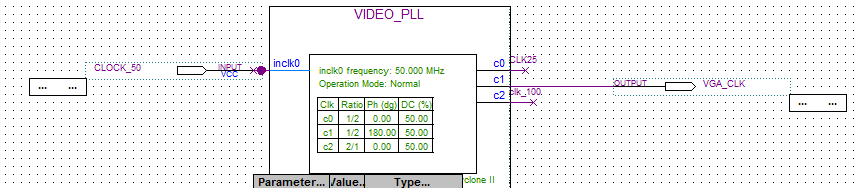
\includegraphics[scale = 0.5]{pll1.png}
\captionof{figure}{This is the first PLL.}
}
\end{minipage}
\medskip

The second one receive signal from 27Mhz and generate 3 signals, all of them are used for providing a adjustable sampling rate, which are 13.5Mhz, 27Mhz and 54Mhz. 

\begin{minipage}[t]{\linewidth}
%\label{fig:main}

{
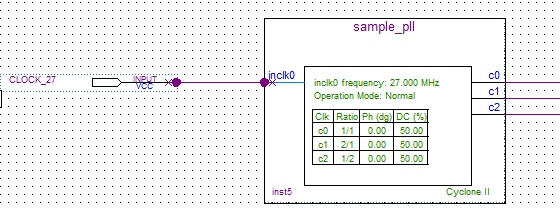
\includegraphics[scale = 0.5]{pll2.png}
\captionof{figure}{This is the second PLL.}
}
\end{minipage}
\medskip

\subsection{University Provided modules}
\subsubsection{The VGA Adaptor Module}

VGA module is used to connect the board with the monitor, below is the schematic snapshot:

\begin{minipage}[t]{\linewidth}
%\label{fig:main}

{
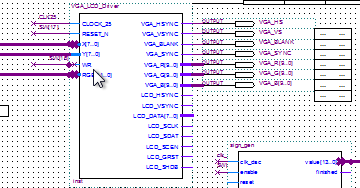
\includegraphics[scale = 1]{vga.png}
\captionof{figure}{This is the VGA Adaptor.}
}
\end{minipage}
\medskip

Although it is a different module, but I use it according to this table \cite{vgaadaptor}.

\subsubsection{The AD-DA Adaptor Module}
AD-DA adaptor module provide a interface for me to control the AD-DA converter. Below is the snapshot of its schematic design:

\begin{minipage}[t]{\linewidth}
%\label{fig:main}

{
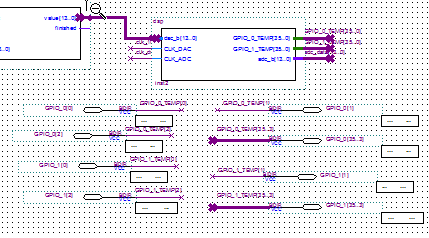
\includegraphics[scale = 1]{adda.png}
\captionof{figure}{This is the AD\-DA Adaptor PLL.}
}
\end{minipage}
\medskip

\subsection{Matlab code}

Beside from the \textit{verilog HDL}, there is roughly $1.5\%$ Matlab code.   
\subsubsection{Matlab code for RAM initialization file} 

Because RAM will need to read its initialing file, two Matlab files are written, one is to generate the background and another one is to generate wave for DA converter.\\

The one for generating the background, it is able to convert an image into Ram initializing file:
\begin{lstlisting}[language=Matlab]
function imgscaled = miffilegen(infile, outfname, numrows, numcols)
%miffilegen('photo.jpg','test.mif',120,160) generate black and white image.

img = imread(infile);
bw = im2bw(img,0.5);

imgresized = imresize(bw, [numrows numcols]);

[rows, cols, ~] = size(imgresized);

imgscaled = imgresized;
imshow(imgscaled*16);

fid = fopen(outfname,'w');

fprintf(fid,'-- %3ux%3u 1bit image color values\n\n',rows,cols);
fprintf(fid,'WIDTH = 1;\n');
fprintf(fid,'DEPTH = %4u;\n\n',rows*cols);
fprintf(fid,'ADDRESS_RADIX = UNS;\n');
fprintf(fid,'DATA_RADIX = UNS;\n\n');
fprintf(fid,'CONTENT BEGIN\n');
imshow(imgscaled);
count = 0;
for r = 1:rows
    for c = 1:cols
%         red = uint16(imgscaled(r,c,1));
%         green = uint16(imgscaled(r,c,2));
%         blue = uint16(imgscaled(r,c,3));
%         color = red*(256) + green*16 + blue;
        fprintf(fid,'%4u : %4u;\n',count, imgscaled(r,c));
        count = count + 1;
    end
end
fprintf(fid,'END;');
fclose(fid);

return
\end{lstlisting}

The code is modified to be able to generate an image directly from Matlab's array, and the standard background is a 160 * 120 image:
\begin{center}
\begin{minipage}[t]{\linewidth}
%\label{fig:main}

{
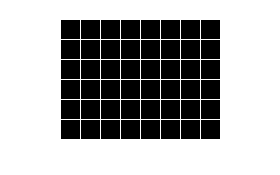
\includegraphics[scale = 1]{temp.png}
\captionof{figure}{This is the background plot.}
}
\end{minipage}
\medskip
\end{center}

\subsubsection{Matlab code for doing measurement}

Those two codes enable us to tell the frequency and amplitude based on the output image on the screen and the switch:
\begin{lstlisting}[language=Verilog]

\end{lstlisting}

\subsubsection{Matlab code for setting up refresh rate}

This code enable us to calculate how much delay is needed to change the refresh rate down to 50hz:
\begin{lstlisting}[language=Verilog]
x = 160;
y = 120;
f = 25*10^6;
t = 1/f;

screen_time = t*x*y;
line_time = t*x;


freq = 48;
one_hz_time = 1/freq;
disp(['to draw a whole screen:',num2str(screen_time) ]);
disp(['to draw a whole line:',num2str(line_time) ]);
disp(['to delay at ',num2str(freq),'hz. 25Mhz needed(positive edge): ',num2str(one_hz_time/t),'. bit needed ',num2str(ceil(log2(one_hz_time/t)))]);
\end{lstlisting}

And it is the output:
\begin{verbatim}
to draw a whole screen:0.000768
to draw a whole line:6.4e-06
to delay at 48hz. 25Mhz needed(positive edge): 520833.3333. bit needed 19
\end{verbatim}



\section{Module Specification}
\subsection{VGA Module}
\subsection{AD Module}
\subsection{DA Module}
\subsection{Plotting Module}
\subsubsection{Drawing Background Module}
\subsubsection{Drawing Wave Module}
\subsubsection{Storing AD Data Module}
\subsubsection{Pause Module}
\subsection{Implementation of the control sequence}


\section{Conclusion and potential works}


\section{Appendix}
\subsection{Problems in the development and the Solution}
\subsubsection{The for loop}
\subsubsection{The FIFO}
\subsubsection{Debugging method}
\subsection{Frequency Table}
\subsection{Amplitude Table}
\subsection{Development History}




\bibliographystyle{plain}
\bibliography{bibliography} 
\end{document}
